\section{Experiments}



We present three experiments. First, we apply generalized CRC (gCRC) to control the false discovery rate in medical question answering, a non-monotonic loss. Second, we apply CPC to constrained active learning, where feedback-loop shifts break exchangeability. Third, we apply CPC to black-box sequence optimization with a language model.

\subsection{Factual Medical Question-Answering}

\textbf{Setup:} We evaluate CRC methods on the MedLFQA dataset \citep{jeong2024olaph}, which aggregates medical question-answering benchmarks. 
We use the dataset of \citet{cherian2024large}, which contains GPT-3.5-Turbo responses, atomic subclaims extracted via GPT-4o, and factuality annotations obtained by checking each subclaim against reference answers. 
Given a confidence score $p(C_{ij} \mid X_i)$ for each subclaim, we filter claims below a threshold $\tau$ and measure the false discovery rate (FDR), the fraction of retained claims that are false, as our loss. 
We measure recall, the fraction of total true claims retained, as our utility metric. Unlike the binary loss used by \citet{mohri2024language} and \citet{cherian2024large}, FDR is non-monotonic in $\tau$, making it a natural test case for gCRC. We compare gCRC against CRC applied to monotonized losses and Learn Then Test (LTT) \citep{angelopoulos2021learn}. See Appendix~\ref{app:medical_qa} for details.

\textbf{Results:} Figure~\ref{fig:MedicalQA} shows FDR and recall across varying risk levels $\alpha$. gCRC controls FDR at or below the target level across all $\alpha$ values while achieving recall at least as high, or often significantly higher, than both the monotonized-losses CRC and LTT baselines. 
Relative to gCRC, LTT is conservative because it uses concentration inequalities to obtain a high-probability guarantee. Monotonized-loss CRC is conservative as a consequence of Jensen's inequality: monotonizing each loss is far more conservative than monotonizing the empirical risk.
% LTT is more conservative due to its use of concentration inequalities to attain a high-probability guarantee (whereas gCRC's guarantees are in expectation), and the conservatism of monotized-losses CRC is a consequence of Jensen's inequality (monotizing losses is far more conservative than monotizing the empirical risk, or average loss value).
% LTT, which uses concentration inequalities for conservative adjustment, is also more conservative than gCRC. 
These results demonstrate that gCRC provides valid risk control for non-monotonic losses where standard CRC may not be valid, and empirically with higher power than baselines.


\subsection{Constrained Active Learning}
\label{subsec:active_learning_experiments}

\textbf{Setup:}
We evaluate CPC in a pool-based active learning setting on three regression datasets: \textbf{Robot Arm Kinematics}, \textbf{Airfoil}, and \textbf{Healthcare Utilization (MEPS)}. Starting from a small initial training set, the learner iteratively selects records from the pool to minimize test MSE.
To create a challenging constrained setting, we construct synthetic feasibility constraints based on the first principal component of the covariate matrix. Records that follow the dominant covariation pattern (high PC1 values) are likely feasible, while records that deviate from this pattern are likely infeasible. Initial training data is sampled from the high-PC1 region, so the learner begins in a high-feasibility region. Uncertainty-based acquisition naturally targets the opposite end of the spectrum.
We fit a Gaussian process regression model and define an acquisition policy via exponential tilting toward posterior variance: $\pi(a) \propto \exp(\lambda \cdot \hat{\sigma}^2_a)$. CPC constrains this policy relative to the source distribution used for initialization. See Appendix~\ref{app:active_learning_details} for details.



\textbf{Results:}
In Figure~\ref{fig:AL_enumerated_options} we present results across all three datasets. CPC successfully controls constraint violation risk at the target $\alpha$ while reducing test MSE. Surprisingly, in some cases the risk-controlled policy attains \textit{lower} test MSE than the unconstrained policy, suggesting that avoiding infeasible regions improves sample efficiency.

\begin{figure*}
    \centering
    \begin{subfigure}{\textwidth}
        
\includegraphics[width=0.9\textwidth]{figures/legend_20251225_MixProp_fixedGetSeeds_0.2Hist_50minOld_solidErrsTrue.pdf}
    \end{subfigure}
    \\
    \begin{subfigure}{0.3\textwidth}
        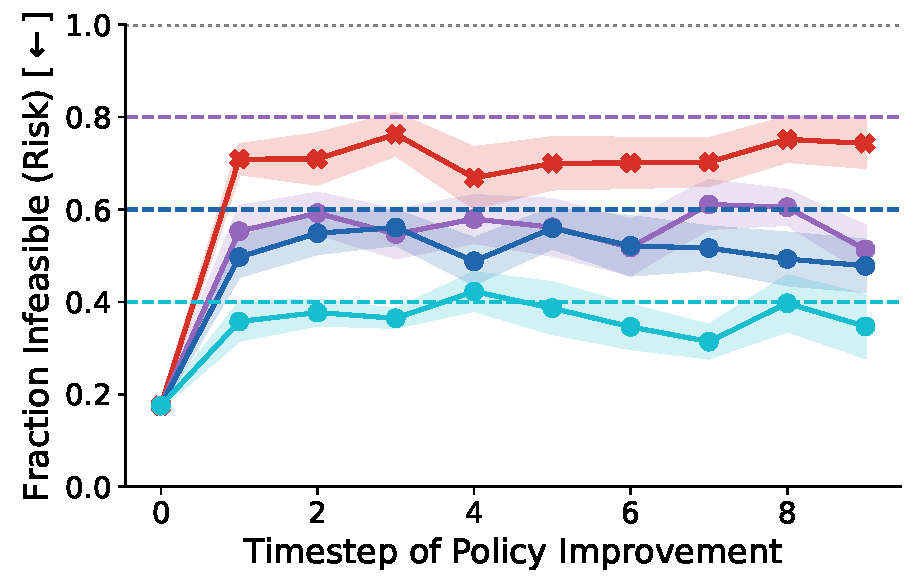
\includegraphics[width=\textwidth]{figures/Infeasibility_20251225_MixProp_fixedGetSeeds_0.2Hist_50minOld_solidErrsTrue_seeds0-9_w24_h4.pdf}
    \end{subfigure}
    \hfill
    \begin{subfigure}{0.3\textwidth}
        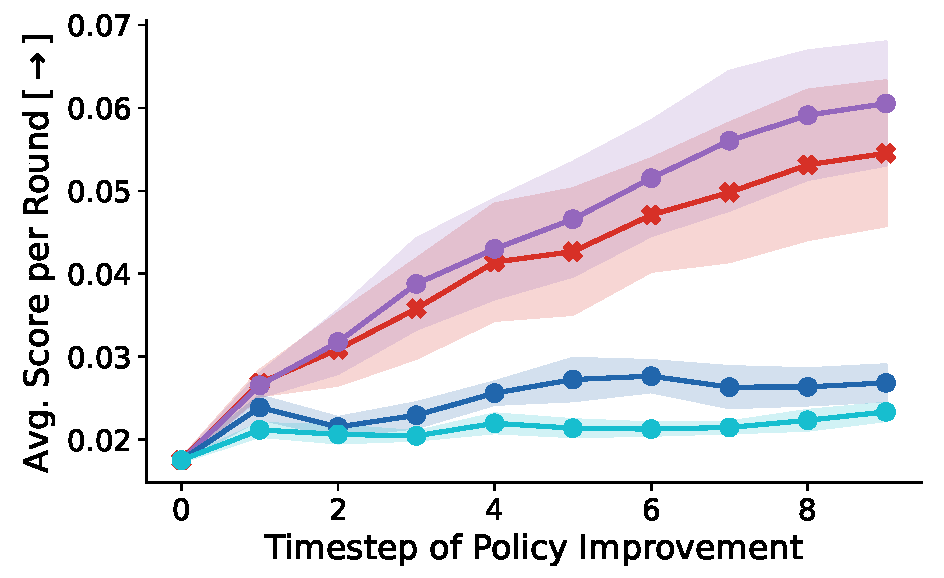
\includegraphics[width=\textwidth]{figures/AvgScores_20251225_MixProp_fixedGetSeeds_0.2Hist_50minOld_solidErrsTrue_seeds0-9_w24_h4.pdf}
    \end{subfigure}
    \hfill
    \begin{subfigure}{0.3\textwidth}
        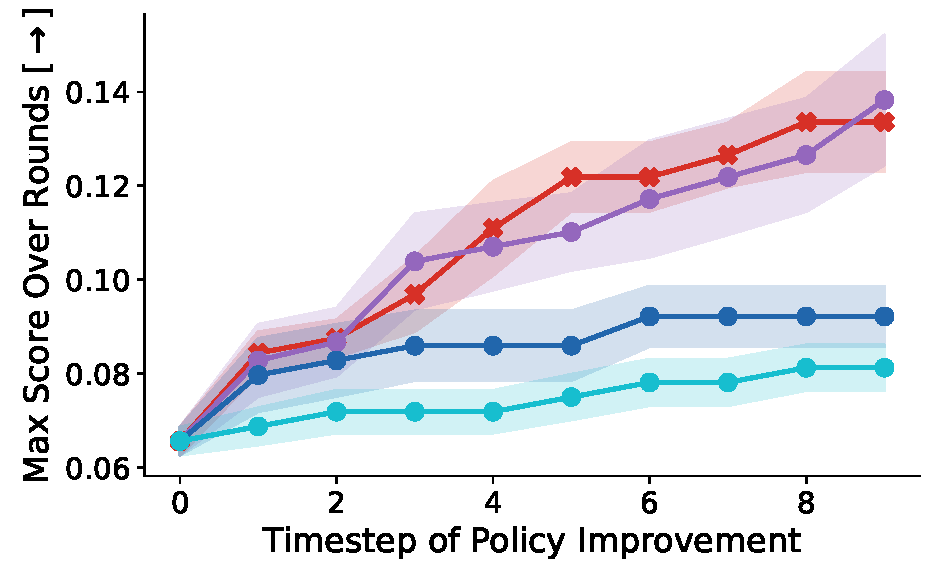
\includegraphics[width=\textwidth]{figures/MaxScores_20251225_MixProp_fixedGetSeeds_0.2Hist_50minOld_solidErrsTrue_seeds0-9_w24_h4.pdf}
    \end{subfigure}
    \caption{
        We apply CPC to constrained black-box sequence optimization scored with Ehrlich functions.
        \textbf{Left:} average infeasibility rate per round.
        \textbf{Center:} average objective value of sequences sampled from the policy.
        \textbf{Right:} best objective value found so far. CPC allows direct control over constraint violation risk via $\alpha$. Without CPC, the infeasibility risk quickly rises to nearly 80\% of policy samples.
        Moderate risk control ($\alpha > 0.6$) stabilizes optimization and improves overall performance by reducing wasted samples on infeasible actions.
    }
    \label{fig:llm_policy_control_results}
\end{figure*}

\subsection{Constrained Black-Box Optimization}
\label{subsec:cpc_LLM_methods}

\textbf{Setup:}
Now consider a more difficult setting, black-box sequence optimization. Here, our goal is to identify a sequence of tokens $a \in \mathcal{X}$ to maximally improve the objective value of a current solution $x \in \mathcal{X}$. We evaluate on Ehrlich functions \citep{chen2025generalists}, synthetic test functions designed to capture the geometric structure of biomolecular sequence optimization problems. We use \textbf{Ehr(32, 32)-4-4-4}: sequences of length 32 over a vocabulary of size 32, with 4 motifs of length 4.
We create an initial data package by running a genetic algorithm from a single feasible solution. We train $\pi_{\theta_0}$ by applying SFT to a Pythia 14M-parameter decoder-only transformer \citep{biderman2023pythia} on improving pairs from the GA history. In later rounds, we sample from the current policy, collect oracle feedback, and fine-tune via DPO. CPC constrains each improved policy $\pi_{\theta_t}$ before sampling. See Appendix \ref{app:sequence_opt} for details.

\textbf{Results:}
In Figure \ref{fig:llm_policy_control_results} we show that CPC effectively controls the risk of generating infeasible sequences while still improving the objective value over time.
Again we find that moderate risk control ($\alpha > 0.6$) can produce controlled policies that slightly \textit{outperform} their uncontrolled counterparts, likely by wasting fewer evaluations on infeasible actions.
